\documentclass[12pt, a4paper, UTF8]{ctexart}
\usepackage{booktabs}
\usepackage{graphicx}
\usepackage[final]{pdfpages}
\usepackage[stable]{footmisc}
\usepackage{threeparttable}
\usepackage{indentfirst}
\setlength{\parindent}{0pt}

\usepackage{minted}
\usepackage{listings}
\usepackage{xcolor}
\lstset{
    rulesepcolor= \color{gray},
    breaklines=true,
    numbers=left,
    numberstyle= \small,
    commentstyle=\color{gray},
    frame=shadowbox
}
\usepackage{subfigure}

\title{基于Android多道作业批处理调度模拟实现}
\author{软件工程2003杜睿}
\date{}

\begin{document}
\tableofcontents
\maketitle

\section{设计目的}
软件体系结构课程设计是在学生系统地学习了《软件设计与体系结构》课程后,按照软件设计模式的基本原理,综合运用所学的知识,设计开发一个应用场景,至少使用三种设计模式解决实际问题。通过对一个实际问题的分析、设计与实现,将原理与应用相结合,使学生学会如何把书本上学到的知识用于解决实际问题,培养学生的动手能力;另一方面,使学生能深入理解和灵活掌握教学内容。

\section{系统设计}

\subsection{设计内容}

模拟实现一个单(多)道批处理系统及其多级调度策略,输入作业序列(提交时间、服务时间、优先级[可选]),输出作业进入内存时间、结束时间、平均周转时间,展示各作业的执行时间线,并对多种调度算法进行性能比较。

\begin{enumerate}
    \item 模拟实现作业调度中先来先服务(FCFS)、短作业优先(SJF)和最高响应比调度(HRRN)算法。每次作业调度时,显示各作业的执行情况(开始执行时间,结束时间,周转时间);最后,计算并列出平均周转时间并对相同情况下不同调度算法进行性能分析比较。
    \item 模拟实现进程调度中基于优先级的时间片轮转调度算法(PRR)和多级反馈队列轮转调度算法(MFQ)。每次进行进程切换时,显示各进程执行情况(剩余时间,进程状态,进程排队情况),最后列出各进程的开始执行时间和结束时间。
\end{enumerate}

\subsection{需求分析}

一个作业从用户提交开始到占有处理机被执行,一般来要由系统三级调度才能实现,即作业调度、内存调度、进程调度。其中最为重要的:
\begin{description}
    \item[作业调度] 主要是完成作业\footnote{用户向计算机提交任务的任务实体,《计算机操作系统教程(第四版)》,清华大学出版社}从\emph{后备状态}到\emph{可执行状态}的转变,即按照某原则,从\emph{外存后备队列}中挑选作业,将其装入\emph{内存}并为其创建进程;
    \item[进程调度] 主要是完成进程从\emph{就绪状态}到\emph{执行(完成)状态}的转变,即按照某策略,从\emph{内存就绪队列}中选取进程,为其分配处理机使其运行。
\end{description}

\begin{table}[htbp]
    \caption{常用的处理机调度策略}
    \centering

    \begin{threeparttable}
        \begin{tabular}{cccccc}
            \toprule
            算法名称           & 主要适用范围       & 默认调度方式         \\
            \midrule
            先来先服务         & 作业调度\&进程调度 & 非抢占式             \\
            短作业(进程)优先 & 作业调度\&进程调度 & 非抢占式             \\
            高响应比优先       & 作业调度           & 非抢占式             \\
            时间片轮转         & 进程调度           & 抢占式(不抢时间片) \\
            多级反馈队列       & 进程调度           & 抢占式(抢占时间片) \\
            \bottomrule
        \end{tabular}

        \zihao{-6}
        \begin{tablenotes}
            \item [*]   调度策略也就是调度算法
        \end{tablenotes}

    \end{threeparttable}
    \qquad
\end{table}
基于上述理论常识,可以做出如下基本假设:
\begin{enumerate}
    \item 作业调度和进程调度是互补共存的层级关系。不考虑内存调度的前提下,实现任何算法,至少要实现两级调度:作业调度及进程调度。
    \item 作业和进程可以合二为一,统一抽象为任务\footnote{作业是提交层面的任务,进程是执行层面的任务,作者注}。不考虑阻塞的前提下,一个任务大致可归为未提交态、收容态、就绪态、运行态及销毁态。
    \item 调度是种将何资源分配给何任务的决策行为。从各级调度的交互上说,调度可以分为:本级进行调度、移交上层调度及委托下层调度。
\end{enumerate}

\subsection{概要设计} \label{v0}

要模拟批处理系统,就须要模拟时钟、任务及其状态、分级调度。

\begin{description}
    \item[时钟] 标定时间流逝的基准,以便执行作业调度、进程调度、性能分析等。每流逝一个单位时间,系统至少要进行一次调度。所以,可以建立“时钟”与“调度器”之间的依赖关系,当时钟发生改变时应该自动通知调度器,调度器接受信息并做出响应。时钟,被称为观察目标;调度器,被称为观察者。一个观察目标可以对应对个观察者,可以根据需要增加和删除观察者。这种设计模式被称为\emph{观察者模式}或\emph{发布-订阅模式}。
    \item[任务] 每个任务都有提交时间、到达时间等属性;运行中任务的剩余时间随时间流逝而减少

        从这种意义说,运行中进程应当观察时间流逝,并自主改变剩余时间字段。换言之,理论上说,任务应当与调度类共同作为时钟的\emph{观察者}。

        任务揉杂作业和进程,集成两者的属性,
        即id、优先级、状态、时钟,提交时间、预计需要时间,到达时间、开始时间、剩余时间、完成时间。

        在模拟逻辑上,状态包含五种类型:未提交、收容、就绪、运行、结束。未提交,代表用户输入作业序列中的提交时间晚于当前时钟时刻;收容,代表作业已提交,进入外存收容队列(外存一般没有容量限制);就绪,代表进程已创建,进入内存就绪队列(内存一般有容量限制);运行,代表进程获得处理机资源,随时间流逝剩余时间递减。
    \item[调度] 任务状态由调度器进行切换;调度是分层级的。

        作业提交与调度细节应当是解耦的,同时为较好地实现“分级”调度,可以将调度器链式组织,各司其职,又保证了作业在各级调度中的传递,直至进程销毁并记录日志。这种思想来源于\emph{职责链模式}。

    \item[机器] 整合时钟、任务、调度,并接受测试样例,提供日志。不同策略在各层级上排列,可以衍生成为多种具体“机器”,例如,以先来先服务作为作业调度、以抢占式多级反馈队列作为进程调度,内存无限制的多道批处理机。为将对象创建和对象使用解耦,可以使用\emph{工厂方法模式}。

        对于各算法性能分析而言,各个“处理机”,由于模拟时减少任务的剩余运行时间,应仅仅保有用户提交序列的副本。即通过拷贝一个已经存在的实例来返回新的实例,而不是新建实例。被复制的实例就是我们所称的“原型”,这个原型是可定制的,例如,只拷贝标识符、提交时间、服务时间和优先级。这种设计模式被称为\emph{原型模式}。
\end{description}

\begin{figure}[htbp]
    \centering
    \includegraphics[height=395pt]{v0-class-compat.png}
    \caption{UML类图(第一版)}
\end{figure}

\newpage
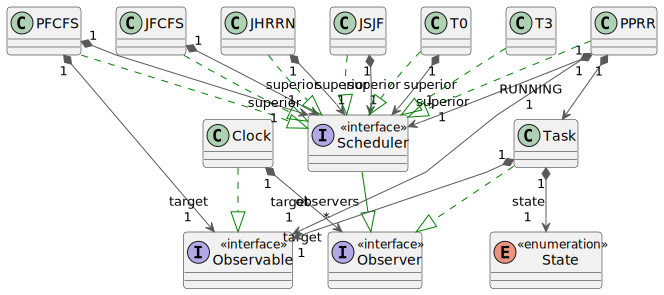
\includepdf{v0-class.pdf}
\newpage

\subsection{质量评审}

基于 \ref{v0} 实现的系统,将存在一个致命缺陷:延时。之所以会延时,主要是因为各个时间观察者对于时间流逝的感知顺序是固定、单向的。
\begin{figure}[htbp]
    \centering
    \includegraphics[height=13.2em]{i-lag.png}
    \caption{通知顺序}
\end{figure}

虽然从层级上说,作业调度高于(先于)进程调度,但是从顺序上说,在单位时间流逝后,有可能出现先作业调度、再进程调度、再作业调度的情况。

\begin{table}[htbp]
    \caption{错误案例(单道批处理系统)}
    \centering
    \begin{tabular}{cccccc}
        \toprule
        时刻   & 收容队列            & 就绪队列            & 备注                 \\
        \midrule
        09:59  & \{\}                & \{[运行,余1分钟]\} & 初始状态             \\
        10:00  & \{\}                & \{[运行,余1分钟]\} & 用户提交新作业       \\
        10:00  & \{[收容,余1分钟]\} & \{[运行,余1分钟]\} & 内存已满|无作业调度 \\
        10:00  & \{[收容,余1分钟]\} & \{[运行,余1分钟]\} & 正在运行|无进程调度 \\
        10:00  & \{[收容,余1分钟]\} & \{[结束,余0分钟]\} & 进程自主修改剩余时间 \\
        \bottomrule
        10:01  & \{[收容,余1分钟]\} & \{[结束,余0分钟]\} & 内存已满|无作业调度 \\
        10:01  & \{[收容,余1分钟]\} & \{\}                & 释放进程(进程调度) \\
        \bottomrule
        10:02  & \{\}                & \{[就绪,余1分钟]\} & 掉入内存(作业调度) \\
        10:02  & \{\}                & \{[运行,余1分钟]\} & 运行进程(进程调度) \\
        10:02  & \{\}                & \{[结束,余0分钟]\} & 进程自主修改剩余时间 \\
        \ldots & \ldots              & \ldots              & \ldots               \\
        \bottomrule
    \end{tabular}
    \qquad
\end{table}

本错误案例中,10:00~10:01处理机竟然处于空闲状态。这是因为:
\begin{itemize}
    \item 进程运行不受进程调度控制,进程调度没有及时将结束进程向上提交;
    \item 进程调度即使向上提交,作业调度也无法预知未来,并为其创建进程。
\end{itemize}

下面提出两种可能的改进方案,并加以分析:
\begin{description}
    \item [调整时间单位] 承认并接受延时的存在,并将时间继续细分。例如,倘若单位设定为“秒”,那么在“分钟”维度上看,延时仿佛并不存在。不过,只要没有无限细分,延时累积最终必将影响结果。
    \item [优化通信机制] 扭转各层对时间流逝固定、单向的感知顺序。拟人地说,各层消息传递机制不能只包含“向上告知”,还要包含“向下问责”。进程调度结束后,倘若可以通知作业调度:“你那里还有什么要我签字处理的吗?”;那么,延时问题说不定就可以迎刃而解。
\end{description}

此外,在上一节的基础上,添加以下前提假设,以便系统实现:时钟的最小颗粒单位为分钟,所有作业均在23:59前提交并结束。
倘若用户要求输入时间单位不统一,可以尝试添加\emph{适配器}。

\section{系统实现}

\subsection{核心实现}
以“多级队列反馈队列”为例,我们需要实现(类图见下页):
\begin{itemize}
    \item 核心组件:
          \begin{itemize}
              \item 任务、状态
              \item 时钟(观察对象)
              \item 提交“调度”、作业调度、进程调度、销毁“调度”(严格意义上说,提交和销毁不属于调度,它们是对定时提交和进程销毁的一种模拟)
          \end{itemize}
    \item 边缘组件:
          \begin{itemize}
              \item 处理机工厂,用不同算法构建各级调度
              \item 测试样例工厂,创建任务并添加至提交“调度”
          \end{itemize}
\end{itemize}

\begin{figure}[htbp]
    \centering
    \includegraphics[height=550pt]{v1-class-compat.png}
    \caption{UML类图(第二版)}
\end{figure}

多级调度各司其职,共同作为批处理系统的重要组成部分发挥作用:

\begin{table}[htbp]
    \caption{常用的处理机调度策略}
    \centering

    \begin{threeparttable}
        \begin{tabular}{cccccc}
            \toprule
            多级调度 & 调度方式                                    & 调度时机                 & 调度次序 & 任务状态   \\
            \midrule
            用户提交 & $\uparrow$                                  & 提交时刻 $\leq$ 当前时刻 & 提交时间 & 未提交     \\
            作业调度 & $\uparrow$                                  & 时间流逝 \& 上层命令     & *        & 收容       \\
            进程调度 & $\uparrow$、$\leftrightarrow$、$\downarrow$ & 时间流逝                 & **       & 就绪、运行 \\
            进程销毁 &                                             &                          &          & 销毁       \\
            \bottomrule
        \end{tabular}

        \zihao{-6}
        \begin{tablenotes}
            \item [1]   $\uparrow$移交上层调度,$\leftrightarrow$本层级调度,$\downarrow$、委托下层调度
            \item [2]   * 提交时间、剩余时间、响应比
            \item [3]   ** 优先级(多级队列优先次序)
        \end{tablenotes}

    \end{threeparttable}
    \qquad
\end{table}

\subsubsection{时钟}
接口:
\begin{minted}[mathescape,
    linenos,
    numbersep=5pt,
    frame=lines,
    gobble=4,
    framesep=2mm]{Java}
    public interface Observable {
        void attachObserver(Observer o);

        void detachObserver(Observer o);

        void notifyObservers();
    }
\end{minted}

具体实现:
\begin{minted}[mathescape,
    linenos,
    numbersep=5pt,
    frame=lines,
    gobble=4,
    framesep=2mm]{Java}
    public class Clock implements Observable {
        public static final int UNIT = 1;
        // main attribute
        public static int minutes = -1;
        // subscribers
        private final List<Observer> observers = new ArrayList<>();

        // TODO timeline logger

        public String getMilestones() {
            return null;
        }

        // increment by one minute
        public void incrementByUnit() {
            minutes += UNIT;
            notifyObservers();
            Log.e("time-line", this + "");
            for (Observer o : observers) {
                Log.e("time-line", o + "");
            }
        }

        // helpers
        public static int parsePatternIntoMinutes(String pattern) {
            String[] parts = pattern.split(":");
            return Integer.parseInt(parts[0]) * 60 + Integer.parseInt(parts[1]);
        }

        public static String generatePatternFromMinutes(int minutes) {
            return String.format(Locale.CHINA, "%02d:%02d", minutes / 60, minutes % 60);
        }


        // constructors & setters
        public Clock(int minutes) {
            Clock.minutes = minutes - 1;
        }

        public Clock(String pattern) {
            minutes = parsePatternIntoMinutes(pattern) - 1;
        }

        // observable implementation
        @Override
        public void attachObserver(Observer o) {
            observers.add(o);
        }

        @Override
        public void detachObserver(Observer o) {
            observers.remove(o);
        }

        @Override
        public void notifyObservers() {
            for (Observer o : observers) {
                o.update(minutes, UNIT);
            }
        }

        // logger
        @Override
        public String toString() {
            return generatePatternFromMinutes(minutes);
        }
    }

\end{minted}

\newpage
\subsubsection{任务}
\begin{minted}[mathescape,
    linenos,
    numbersep=5pt,
    frame=lines,
    gobble=4,
    framesep=2mm]{Java}
    public class Task implements Cloneable {
        // auto-increment
        private static int COUNTER = 0;
    
        // universal attribute
        private final int id;
        private int priority = 0;
        private State state = State.NULL;
    
        // exclusive for job scheduling
        private final int jobSubmitTime;
        private final int estimatedRequireTime;
    
        // exclusive for process scheduling
        private int processLeftTime;
        private int processArriveTime = -1;
        private int processStartTime = -1;
        private int processCompleteTime = -1;
    
        public Task(int id, int priority, int jobSubmitTime, int estimatedRequireTime) {
            this.id = id;
            this.priority = priority;
            this.jobSubmitTime = jobSubmitTime;
            this.estimatedRequireTime = estimatedRequireTime;
            this.processLeftTime = estimatedRequireTime;
        }
    
        public Task(int priority, int jobSubmitTime, int estimatedRequireTime) {
            this.id = COUNTER++;
            this.priority = priority;
            this.jobSubmitTime = jobSubmitTime;
            this.estimatedRequireTime = estimatedRequireTime;
            this.processLeftTime = estimatedRequireTime;
        }
    
        public Task(int jobSubmitTime, int estimatedRequireTime) {
            this.id = COUNTER++;
            this.jobSubmitTime = jobSubmitTime;
            this.estimatedRequireTime = estimatedRequireTime;
            this.processLeftTime = estimatedRequireTime;
        }
    
        public void decrementLeftTime(int currentTime, int elapseUnit) {
            if (isRunning()) {
                this.processLeftTime -= elapseUnit;
                if (processLeftTime <= 0) {
                    toggleTerminated(currentTime);
                }
            }
        }
    
        public void incrementPriority(int diff) {
            this.priority += diff;
        }
    
        public void toggleBackup() {
            this.state = State.BACKUP;
        }
    
        public void toggleReady(int arriveTime) {
            this.state = State.READY;
            this.processArriveTime = arriveTime;
        }
    
        public void toggleReReady() {
            this.state = State.READY;
        }
    
        public void toggleTerminated(int completeTime) {
            this.state = State.TERMINATED;
            this.processCompleteTime = completeTime;
        }
    
        public void toggleRunning(int startTime) {
            this.state = State.RUNNING;
            if (processStartTime == -1) {
                this.processStartTime = startTime;
            }
        }
    
        public boolean isBackup() {
            return this.state == State.BACKUP;
        }
    
        public boolean isReady() {
            return this.state == State.READY;
        }
    
        public boolean isRunning() {
            return this.state == State.RUNNING;
        }
    
        public boolean isTerminated() {
            return this.state == State.TERMINATED;
        }
    
        public int getId() {
            int factor = (isRunning()) ? (-1) : (1);
            return id * factor;
        }
    
        public int getJobSubmitTime() {
            int factor = (isRunning()) ? (-1) : (1);
            return jobSubmitTime * factor;
        }
    
        public int getPriority() {
            int factor = (isRunning()) ? (-1) : (1);
            return priority * factor;
        }
    
        public int getProcessLeftTime() {
            int factor = (isRunning()) ? (-1) : (1);
            return processLeftTime * factor;
        }
    
        public int getProcessArriveTime() {
            int factor = (isRunning()) ? (-1) : (1);
            return processArriveTime * factor;
        }
    
        public int getProcessStartTime() {
            int factor = (isRunning()) ? (-1) : (1);
            return processStartTime * factor;
        }
    
        public int getProcessCompleteTime() {
            int factor = (isRunning()) ? (-1) : (1);
            return processCompleteTime * factor;
        }
    
        public int getEstimatedRequireTime() {
            return estimatedRequireTime;
        }
    
        public double getResponseRate(int currentTime) {
            int factor = (isRunning()) ? (-1) : (1);
            return (1 + ((1.0 * currentTime - jobSubmitTime) 
            / estimatedRequireTime)) * factor;
        }
    
        public int getRoundTime() {
            int factor = (isRunning()) ? (-1) : (1);
            return (processCompleteTime - jobSubmitTime) * factor;
        }
    
        public String toString() {
            return String.format("{%d,%s,%s}", id, state, 
                Clock.generatePatternFromMinutes(processLeftTime));
        }
    
        public Object clone() {
            return new Task(this.id, this.priority, this.jobSubmitTime, 
                this.estimatedRequireTime);
        }
    }    
\end{minted}

\newpage
\subsubsection{机器}
\begin{minted}[mathescape,
    linenos,
    numbersep=5pt,
    frame=lines,
    gobble=4,
    framesep=2mm]{Java}
    public class Machine {
        private String TAG;
        private Clock clock;
        private Scheduler submitImitator;
        private Scheduler jobScheduler;
        private Scheduler processScheduler;
        private Scheduler landfilImitator;

        public void run() {
            build();
            while (!(submitImitator.isEmpty() 
                && jobScheduler.isEmpty() && processScheduler.isEmpty())) {
                clock.incrementByUnit();
            }

            ((T3) landfilImitator).getFinalSnapShot();
        }

        // getters
        public float getAverageRoundTime() {
            return ((T3) landfilImitator).getAverageRoundTime();
        }

        public String getTAG() {
            return TAG;
        }

        public String getFinalSnapShot() {
            return ((T3) landfilImitator).getFinalSnapShot();
        }

        public Object[] getFinalSnapShotTasks() {
            return ((T3) landfilImitator).getFinalSnapShotTasks();
        }

        // setters
        public Machine setQuantum(int quantum) {
            if (processScheduler.getClass().equals(PPRR.class)) {
                ((PPRR) processScheduler).setQuantum(quantum);
            }
            return this;
        }

        public Machine setFactor(int factor) {
            if (processScheduler.getClass().equals(PMFQ.class)) {
                ((PMFQ) processScheduler).setFactor(factor);
            } else if (processScheduler.getClass().equals(PMFQB.class)) {
                ((PMFQB) processScheduler).setFactor(factor);
            }
            return this;
        }

        public Machine setTrial(List<Task> tasks) {
            int starter = Integer.MAX_VALUE;
            for (Task task : tasks) {
                // FIXME prototype
                submitImitator.add((Task) task.clone());
                starter = Math.min(starter, task.getJobSubmitTime());
            }
            this.clock = new Clock(starter);
            return this;
        }

        public Machine setTAG(String TAG) {
            this.TAG = TAG;
            return this;
        }

        public Machine setClock(Clock clock) {
            this.clock = clock;
            return this;
        }

        public Machine setSubmitImitator(Scheduler submitImitator) {
            this.submitImitator = submitImitator;
            return this;
        }

        public Machine setJobScheduler(Scheduler jobScheduler) {
            this.jobScheduler = jobScheduler;
            return this;
        }

        public Machine setProcessScheduler(Scheduler processScheduler) {
            this.processScheduler = processScheduler;
            return this;
        }

        public Machine setLandfilImitator(Scheduler landfilImitator) {
            this.landfilImitator = landfilImitator;
            return this;
        }





        // Observer & Chain of Responsibility
        private void build() {
            submitImitator.observe(clock);
            jobScheduler.observe(clock);
            processScheduler.observe(clock);
            landfilImitator.observe(clock);
            submitImitator.setSuperior(jobScheduler);
            jobScheduler.setSuperior(processScheduler);
            processScheduler.setSuperior(landfilImitator);
            landfilImitator.setInferior(processScheduler);
            processScheduler.setInferior(jobScheduler);
            jobScheduler.setInferior(submitImitator);
        }
    }

\end{minted}

\newpage
\subsubsection{机器建造者}
接口:
\begin{minted}[mathescape,
    linenos,
    numbersep=5pt,
    frame=lines,
    gobble=4,
    framesep=2mm]{Java}
    public interface MachineBuilder {
        Machine build();
    }
\end{minted}

具体实现,以先来先服务为例:
\begin{minted}[mathescape,
    linenos,
    numbersep=5pt,
    frame=lines,
    gobble=4,
    framesep=2mm]{Java}
    public class FCFSBuilder implements MachineBuilder {
    public Machine build() {
        return new Machine()
                .setTAG("FCFS")
                .setClock(new Clock("00:00"))
                .setSubmitImitator(new T0())
                .setJobScheduler(new JFCFS())
                .setProcessScheduler(new PFCFS().setLIMIT(1))
                .setLandfilImitator(new T3());
        }
    }
\end{minted}

\newpage
\subsubsection{作业调度}
实现单道批处理系统,作业调度分别使用“先来先服务算法”、“短作业优先算法”、“高响应比优先算法”,进程调度统一使用“先来先服务算法”。

\begin{figure}[htbp]
    \centering
    \includegraphics[height=232.5pt]{t1-class.png}
    \caption{作业调度层}
\end{figure}

作业调度的职责是按照一定的策略,向进程调度提交任务(填入内存)。FCFS、HRRN、SJF的不同主要体现于调度次序,即优先队列的比较方式。本节主要以高响应比优先实现为例,介绍抽象调度类与作业调度层。

\begin{minted}[mathescape,
    linenos,
    numbersep=5pt,
    frame=lines,
    gobble=4,
    framesep=2mm]{Java}
    public abstract class Scheduler implements Observer {
        protected int LIMIT = Integer.MAX_VALUE;
        protected Scheduler superior = null;
        protected Scheduler inferior = null;
    
        public void setLIMIT(int LIMIT) {this.LIMIT = LIMIT;}
    
        public void setSuperior(Scheduler superior) {this.superior = superior;}
    
        public void setInferior(Scheduler inferior) {this.inferior = inferior;}
    
        @Override
        public void observe(Observable target) {target.attachObserver(this);}
    
        @Override
        public void forsake(Observable target) {target.detachObserver(this);}
    
        public abstract boolean add(Task t);
    
        public abstract boolean reportToSuperior();
    
        public abstract boolean notifyToInferior();
    
        public abstract boolean rebase();
    
        public abstract int size();
    
        public abstract boolean isEmpty();
    
        public abstract void shuffle();
    }
\end{minted}

下面对于各个接口,分别解释具体实现:

\begin{lstlisting}[language={java},caption={收容队列(基于响应比的优先队列)}]
private PriorityQueue<Task> queue = new PriorityQueue<>(new Comparator<Task>() {
    @Override
    public int compare(Task o1, Task o2) {
        return (o2.getResponseRate(Clock.minutes) - o1.getResponseRate(Clock.minutes) > 0) ? (1) : (-1);
    }
});
\end{lstlisting}

\begin{lstlisting}[language={java},caption={调度方式(向上提交),调度时机(时间流逝)}]
@Override
public void update(int currentTime, int elapseUnit) {
    boolean flag = true;
    while (queue.peek() != null && flag) {
        flag = reportToSuperior();
    }
}
\end{lstlisting}

\begin{lstlisting}[language={java},caption={添加作业(收容状态)}]
@Override
public boolean add(Task t) {
    if (queue.size() >= LIMIT)
        return false;

    t.toggleBackup();
    queue.offer(t);
    return true;
}
\end{lstlisting}

\begin{lstlisting}[language={java},caption={模拟为作业创建进程,装填进入内存}]
@Override
public boolean reportToSuperior() {
    if (superior == null || queue.isEmpty())
        return false;

    shuffle();
    if (!superior.add(queue.peek()))
        return false;

    return rebase();
}
\end{lstlisting}

\begin{lstlisting}[language={java},caption={在本层队列中移除任务}]
@Override
public boolean rebase() {
    if (queue.isEmpty())
        return false;

    queue.poll();
    return true;
}
\end{lstlisting}

\begin{lstlisting}[language={java},caption={响应比动态变化,刷新队列顺序}]
@Override
public void shuffle() {
    if (queue.size() >= 2) {
        queue.offer(queue.poll());
    }
}
\end{lstlisting}

需要特别说明的是,短作业优先(SJF, Shortest Job First)也有抢占式的版本,通常被称为最短剩余时间优先。即,每当就绪队列改变时都需要进行调度,如果新到达的进程剩余时间比当前运行进程剩余时间更短,则由新进程抢占处理机,当前运行进程重新回到就绪队列。

\subsubsection{进程调度}
实现多道批处理系统(容量无限),作业调度统一使用“先来先服务”,进程调度分别使用“基于动态优先级的时间片轮转法”、“多级反馈队列法”。

\begin{figure}[htbp]
    \centering
    \includegraphics[scale=0.18]{t2-class.png}
    \caption{进程调度层}
\end{figure}

本节主要介绍四种算法的实现异同。共性,例如,只有进程调度会通知下层。
\begin{lstlisting}[language={java},caption={命令下层再次进行调度}]
@Override
public boolean notifyToInferior() {
    if (inferior == null)
        return false;

    return inferior.reportToSuperior();
}
\end{lstlisting}

此外,进程调度的大体框架如下:
\begin{figure}[htbp]
    \centering
    \includegraphics{i-process-fcfs.png}
    \caption{进程调度(以先来先服务为例)}
\end{figure}

不过,不同算法实现细节有所差别,下面结合代码进行分析。这里采用改进通信机制的方式避免延时问题,即,进程调度后,若向上提交销毁进程导致内存存在空余,则通知作业调度并允许其提交新的进程。

\begin{lstlisting}[language={java},caption={先来先服务}]
private boolean leisure = true;
private PriorityQueue<Task> queue = new PriorityQueue<>(Comparator.comparingInt(Task::getProcessArriveTime));

@Override
public void update(int currentTime, int elapseUnit) {
    shuffle();

    // existing a running process
    if (!leisure) {
        queue.peek().decrementLeftTime(currentTime, elapseUnit);
        if (queue.peek().isTerminated()) {
            reportToSuperior();
            leisure = true;
        } else {
            leisure = false;
        }
    }

    // needy for a ready process
    if (leisure) {
        notifyToInferior();
        if (queue.peek() != null) {
            queue.peek().toggleRunning(currentTime);
            leisure = false;
        }
    }
}
\end{lstlisting}

基于动态优先级的时间片轮转要求对时间片动态判定修改。此外,程序没有记录运行进程的引用,所以必须通过tricks保证运行进程优先级永远最高。

\begin{lstlisting}[language={java},caption={Getter(以优先级为例)}]
public int getPriority() {
    int factor = (isRunning()) ? (-1) : (1);
    return priority * factor;
}
\end{lstlisting}

\begin{lstlisting}[language={java},caption={基于动态优先级的时间片轮转}]
private boolean leisure = true;
private int quantum = 2;
private int dynamicTimeSlice = quantum;
private PriorityQueue<Task> queue = new PriorityQueue<>(new Comparator<Task>() {
    @Override
    public int compare(Task o1, Task o2) {
        return (o1.getPriority() - o2.getPriority() != 0) ? (o1.getPriority() - o2.getPriority()) : (o1.getJobSubmitTime() - o2.getJobSubmitTime());
        // return o1.getPriority() - o2.getPriority();
    }
});

public void setQuantum(int quantum) {
    this.quantum = quantum;
}

public void update(int currentTime, int elapseUnit) {
    shuffle();

    // existing a running process within the last minute
    if (!leisure) {
        queue.peek().decrementLeftTime(currentTime, elapseUnit);
        dynamicTimeSlice -= elapseUnit;
        // terminated
        if (queue.peek().isTerminated()) {
            queue.peek().incrementPriority(2);
            reportToSuperior();
            // reset time slice
            leisure = true;
        } else if (queue.peek().isRunning()) {
            // brute-force offline
            if (dynamicTimeSlice == 0) {
                queue.peek().incrementPriority(2);
                queue.peek().toggleReReady();
                shuffle();
                leisure = true;
            }
            // slice is still adequate for continuous running
            else {
                leisure = false;
            }
        }
    }

    // needy for a ready process
    if (leisure) {
        dynamicTimeSlice = quantum;
        notifyToInferior();
        if (queue.peek() != null) {
            queue.peek().toggleRunning(currentTime);
            leisure = false;
        }
    }

}
\end{lstlisting}

多级反馈队列法:设置多级就绪队列,各级队列优先级从高到低,时间片由小到大。新进程到达时,先进入第一级队列,按“先来先服务”原则排队等待。若时间片用完进程仍未结束,则将该进程移入下级队列队尾(直至最后一级)。只有第$k$级队列为空,才会为$k+1$级队头进程分配时间片。

\begin{lstlisting}[language={java},caption={多级反馈队列(数据结构)}]
private List<Deque<Task>> queues = new ArrayList<>();
private boolean leisure = true;
private int busyIndex = 0;
private int quantum = 1;
private int dynamicTimeSlice = quantum;

public PMFQ() {
    Deque<Task> top = new ArrayDeque<>();
    queues.add(top);
    Deque<Task> mid = new ArrayDeque<>();
    queues.add(mid);
    Deque<Task> btm = new ArrayDeque<>();
    queues.add(btm);
\end{lstlisting}

多级反馈队列法同样可分为抢占式和非抢占式,这两种实现的主要区别在于“调度时机”。假设当前运行进程优先级并非顺位第一,即使时间片未运行完,抢占式调度也会收回剩余时间片使优先级更高的新进程获得处理机资源,并将被抢占处理机的进程重新放回原队列队尾。而非抢占式调度须要等时间片轮转才可以调度。
\begin{lstlisting}[language={java},caption={多级反馈队列(非抢占式调度)}]
@Override
public void update(int currentTime, int elapseUnit) {
    // existing a running process within the last minute
    if (!leisure) {
        Deque<Task> queue = queues.get(busyIndex);
        queue.peek().decrementLeftTime(currentTime, elapseUnit);
        dynamicTimeSlice -= elapseUnit;
        // terminated
        if (queue.peek().isTerminated()) {
            reportToSuperior();
            // reset time slice
            leisure = true;
        } else if (queue.peek().isRunning()) {
            // brute-force offline
            if (dynamicTimeSlice == 0) {
                queue.peek().toggleReReady();
                int nextIndex = Math.min(busyIndex + 1, 2);
                // next level or bottom
                queues.get(nextIndex).offer(queue.poll());
                leisure = true;
            }
            // slice is still adequate for continuous running
            else {
                leisure = false;
            }
        }
    }

    // needy for a ready process
    if (leisure) {
        notifyToInferior();
        // somebody ready
        if (nextBusyIndex() != -1) {
            busyIndex = nextBusyIndex();
            quantum = (int) Math.pow(2, busyIndex);
            dynamicTimeSlice = quantum;

            Deque<Task> queue = queues.get(busyIndex);
            queue.peek().toggleRunning(currentTime);
            leisure = false;
        }
    }
}
\end{lstlisting}

\begin{lstlisting}[language={java},caption={多级反馈队列(抢占式调度)}]
@Override
public void update(int currentTime, int elapseUnit) {
    // existing a running process within the last minute
    if (!leisure) {
        Deque<Task> queue = queues.get(busyIndex);
        queue.peek().decrementLeftTime(currentTime, elapseUnit);
        dynamicTimeSlice -= elapseUnit;
        // terminated
        if (queue.peek().isTerminated()) {
            reportToSuperior();
            // reset time slice
            leisure = true;
        } else if (queue.peek().isRunning()) {
            // brute-force offline
            if (dynamicTimeSlice == 0) {
                queue.peek().toggleReReady();
                int nextIndex = Math.min(busyIndex + 1, 2);
                // next level or bottom
                queues.get(nextIndex).offer(queue.poll());
                leisure = true;
            }
            // slice is still adequate for continuous running
            else {
                // nobody can forcibly occupy
                if (nextBusyIndex() == busyIndex) {
                    leisure = false;
                } else {
                    // FIXME
                    queue.peek().toggleReReady();
                    queue.offer(queue.poll());
                    leisure = true;
                }
            }
        }
    }

    if (leisure) {
        notifyToInferior();
        if (nextBusyIndex() != -1) {
            busyIndex = nextBusyIndex();
            quantum = (int) Math.pow(2, busyIndex);
            dynamicTimeSlice = quantum;

            Deque<Task> queue = queues.get(busyIndex);
            queue.peek().toggleRunning(currentTime);
            leisure = false;
        }
    }
}
\end{lstlisting}

\subsection{边缘实现}

选择使用Android移动平台部署应用,以省去云服务器环境搭建。

\subsubsection{依赖配置}

\begin{minted}{groovy}
android {
    namespace 'edu.wust.durui'
    compileSdk 32
    defaultConfig {
        vectorDrawables.useSupportLibrary = true
        multiDexEnabled true
        applicationId "edu.wust.durui"
        minSdk 29
        ...
    }
    ...
    viewBinding {
        enabled = true
    }
    dataBinding {
        enabled = true
    }
}
dependencies {
    ...
    implementation 'com.google.android.material:material:1.6.1'
    implementation "androidx.lifecycle:lifecycle-livedata-ktx:2.4.1"
    implementation "androidx.lifecycle:lifecycle-viewmodel-ktx:2.5.1"
    implementation "androidx.multidex:multidex:2.0.1"
    implementation "androidx.fragment:fragment:1.5.5"
    implementation 'com.github.blackfizz:eazegraph:1.2.2@aar'
    implementation 'com.nineoldandroids:library:2.4.0'
    implementation 'com.github.vipulasri:timelineview:1.1.5'
}
\end{minted}

\subsubsection{架构设计}
谷歌在安卓开发者文档中强调,“应用架构定义了应用的各个部分之间的界限以及每个部分应承担的职责”,推荐按照下列原则设计应用架构:
\begin{enumerate}
    \item 关注点分离。基于界面的类(Activity或Fragment)只应该包含界面和交互。这些类应尽可能保持精简,以避免产生与组件生命周期相关的问题,并提高可测试性。毕竟,操作系统可能会根据内存不足等系统条件随时销毁它们,所以,最好避免在Activity或Fragment编写所有代码。
    \item 数据驱动界面。数据模型应独立于界面或其他组件。持久性模型是理想之选,因为如果 Android 操作系统销毁应用以释放资源,用户也不会丢失数据。
    \item 单一数据源和单向数据流(Unidirectional Data Flow)。一定条件下,只有唯一的数据所有者(Signle Source Of Truth)可以修改数据。在离线优先应用中,应用数据的单一数据源通常是数据库。
\end{enumerate}

基于上述架构原则,每个应用应至少有两个层:界面层和数据层。
\begin{description}
    \item[界面层] 负责展示数据,更新数据,一般对应Activity或Fragment类。
    \item[数据层] 包含业务逻辑,包含应用创建、存储和更改数据的规则,向应用的其余部分公开数据,一般对应一个数据类。
    \item[网域层] 位于界面与数据层之间的可选层,负责封装复杂的业务逻辑,一般该层中的类通常称为用例(UseCase),每个用例都应仅负责单个功能。
\end{description}

关系到核心架构的两个关键概念是“MVVM”和“MutableLiveData”。
\begin{description}
    \item[MVVM]
        MVVM(Model-View-ViewModel)是一种应用架构,它将应用程序分为三个部分:Model(模型层),View(视图层)和ViewModel(视图模型层)。View仅负责显示数据并接收用户输入,ViewModel仅负责处理业务逻辑并将数据从Model传递到View。

    \item[MutableLiveData]
        LiveData是生命周期感知型组件,它只会在组件处于激活状态时才会回调相应的方法,从而刷新界面。从软件设计模式的角度说,它原生支持\emph{观察者模式},能够在数据发生变化时通知观察者(Activity或Fragment等)进行相应的处理。
\end{description}

\subsubsection{核心技术}
\begin{description}
    \item[Fragment]
        Fragment组件介于Activity和View:一方面,它未继承Context,无法独立存在,必须作为宿主视图的一部分;可另一方面,它又可以定义管理自己的布局,具有自己的生命周期(Lifecycle)。
    \item[RecyclerView] 核心视图组件之一,用于显示大量数据。
    \item[DatePicker] 核心视图组件之一。日期选择控件的主要功能是向用户提供包含年、月、日的日期数据并允许用户对其修改。
    \item[EazeGraph]
        核心视图组件之一。轻量级的图表库\footnote{https://github.com/paulroehr/EazeGraph},支持生成四种图表:条形图,层叠柱状图,饼状图,折线图。
    \item[TimelineView]
        核心视图组件之一。轻量级时间视图库\footnote{https://github.com/vipulasri/Timeline-View},支持呈现时间线,应用广泛,如物流追踪历史节点等。

\end{description}

\subsection{原型设计}

\begin{figure}[htbp]
    \centering
    \includegraphics[scale=0.08]{i-prototype.png}
    \caption{界面原型设计图}
\end{figure}

\newpage
\section{系统测试}

\subsection{测试用例}
\begin{table}[htbp]
    \caption{测试用例(短作业优先,平均周转时间1.550h)}
    \centering
    \begin{tabular}{cccccc}
        \toprule
        作业 & 进入时刻 & 运行时间(小时) & 开始时刻 & 完成时刻 & 周转时间(小时) \\
        \midrule
        1    & 08:00    & 2.00             & 08:00    & 10:00    & 2.00             \\
        2    & 08:30    & 0.50             & 10:18    & 10:48    & 2.30             \\
        3    & 09:00    & 0.10             & 10:00    & 10:06    & 1.10             \\
        4    & 09:30    & 0.20             & 10:06    & 10:18    & 0.80             \\
        \bottomrule
    \end{tabular}
    \qquad
\end{table}

\begin{table}[htbp]
    \caption{测试用例(高响应比优先,平均周转时间1.625h)}
    \centering
    \begin{tabular}{cccccc}
        \toprule
        作业 & 进入时刻 & 运行时间(小时) & 开始时刻 & 完成时刻 & 周转时间(小时) \\
        \midrule
        1    & 08:00    & 2.00             & 08:00    & 10:00    & 2.00             \\
        2    & 08:30    & 0.50             & 10:06    & 10:36    & 2.10             \\
        3    & 09:00    & 0.10             & 10:00    & 10:06    & 1.10             \\
        4    & 09:30    & 0.20             & 10:36    & 10:48    & 1.30             \\
        \bottomrule
    \end{tabular}
    \qquad
\end{table}

\begin{table}[htbp]
    \caption{测试用例(248抢占式多级反馈队列)}
    \centering
    \begin{tabular}{cccccc}
        \toprule
        作业 & 进入时刻 & 服务时间 & 完成时刻 & 周转时间 \\
        \midrule
        A    & 0        & 7        & 11       & 11       \\
        B    & 5        & 4        & 19       & 14       \\
        C    & 7        & 13       & 30       & 23       \\
        D    & 12       & 9        & 33       & 21       \\
        \bottomrule
    \end{tabular}
    \qquad
\end{table}

\subsection{运行结果}
见尾页。

\begin{figure}[h]
    \centering
    \subfigure[任务列表]{
        \begin{minipage}[t]{0.42\linewidth}
            \centering
            \includegraphics[width=2in]{app-list.jpg}
        \end{minipage}
    }
    \subfigure[时刻输入]{
        \begin{minipage}[t]{0.42\linewidth}
            \centering
            \includegraphics[width=2in]{app-clock.jpg}
        \end{minipage}%
    }
    \quad

    \subfigure[性能比较]{
        \begin{minipage}[t]{0.42\linewidth}
            \centering
            \includegraphics[width=2in]{app-statistics.jpg}
        \end{minipage}
    }
    \subfigure[时间线]{
        \begin{minipage}[t]{0.42\linewidth}
            \centering
            \includegraphics[width=2in]{app-timeline.jpg}
        \end{minipage}
    }
    \centering
    \caption{运行截图}
\end{figure}

\section{设计总结}

宏观而言,软件设计是针对软件的功能需求、可维护性和可复用性。例如,如果客户要求实现基于“短作业优先”的作业调度和基于“(抢占式)多级反馈队列”的\emph{两道批处理系统},本系统及其容易扩展。~\\

微观而言,以下设计模式我深有体会:

\begin{description}
    \item[观察者模式] 定义了一种一对多的依赖关系,让多个观察者对象同时监听(订阅)某一个主题对象,当主题对象发生变化时,它的所有依赖者(观察者)都会自动收到通知并更新。

        在这种情形下,我们认为观察者是平等的,更新顺序是固定的。在本系统设计中,倘若仅仅使用本模式,将导致延时。

    \item[职责链模式] 使多个对象都有机会处理请求,从而避免请求的发送者和接收者之间的耦合关系。将这些对象连成一条链,并沿该链传递处理请求。

        作业调度是高级调度,负责辅存与内存间的调度;进程调度是低级调度,负责内存与处理器间的调度。两者天然具有职责链关系。

        为了避免“延时”问题,我引入了“双向职责链模式”,即作业调度不止可以向进程调度提交作业,进程调度也可以通知作业调度允许提交作业。

    \item[工厂方法模式] 定义了一个创建对象的抽象方法,由子类决定要实例化的类。工厂方法模式将对象的实例化推迟到子类。

        机器多种多样,如果要进行各算法间的比较,就要创建多种机器。本系统使用工厂方法,实现创建与使用的结耦。

    \item[原型模式] 拷贝这些原型创建新的对象。

        对于各算法性能分析而言,各个“处理机”,由于模拟时减少任务的剩余运行时间,应仅仅保有用户提交序列的副本。即通过拷贝一个已经存在的实例来返回新的实例,而不是新建实例。

\end{description}
总之,在使用“软件设计模式”时应该活学活用,切忌生搬硬套。最终目的都是让程序低耦合、高复用、高内聚、易扩展、易维护。

\end{document}